%%%%%%%%%%%%%%%%%%%%%%%%%%%%%%%%%%%%%%%%%%%%%%%%%%%%%%%%%%%%%%%%%
% Contents : The creation of a report chapter
% $Id : grisbi-manuel-reports-creation.tex, v 0.4 2002/10/27 Daniel Cartron
% $Id : grisbi-manuel-reports-creation.tex, v 0.5.0 2004/06/01 Loic Breilloux
% $Id : grisbi-manuel-reports-creation.tex, v 0.6.0 2011/11/17 Jean-Luc Duflot
% $Id : grisbi-manuel-reports-creation.tex, v 0.8.9 2012/04/27 Jean-Luc Duflot
% $Id : grisbi-manuel-reports-creation.tex, v 1.0 2014/02/12 Jean-Luc Duflot
%%%%%%%%%%%%%%%%%%%%%%%%%%%%%%%%%%%%%%%%%%%%%%%%%%%%%%%%%%%%%%%%%

\chapter{Création d'un état\label{reportscreation}}


Ce chapitre détaille la création d'un état à partir de modèles, au moyen de la  fenêtre de création/modification. Pour toute autre action sur les états, consultez le chapitre \vref{reports}, \menu{États}.

% espace pour changement de thème
\vspacepdf{5mm}
La création d'un état se compose de quatre étapes :

\begin{enumerate}
 \item le choix du modèle de l'état de départ : \indexword{vierge}\index{etat@état !vierge}, \indexword{préformaté}\index{etat@état !préformaté} ou \indexword{préexistant}\index{etat@état !préexistant} ; 
 \item la sélection des données que vous souhaitez extraire de votre fichier de comptes ; suivant le modèle choisi, Grisbi ne sélectionne que certaines données ; par votre sélection, vous ajouterez les données qui vous intéressent, et retirerez celles qui ne vous intéressent pas ;
 \item l'organisation des données ; vous pouvez utiliser jusqu'à quatre niveaux de regroupement, chacun de ces niveaux étant imbriqué dans le niveau supérieur ;
 \item l'affichage des données de la façon adéquate (\gls{tri}, type d'information affichée, \indexword{titres des colonnes}\index{titre !colonnes}, etc.).
\end{enumerate}

À la fin, quand vous en avez terminé avec toutes les sélections, l'organisation et l'affichage des données, et que vous avez bien donné un nom à votre état, vous pouvez valider ce nouvel état par le bouton \menu{Valider} dans la fenêtre de création/modification. Votre nouvel état apparaîtra alors dans la liste des états, dans le panneau de navigation.


\section{Choix du modèle de l'état de départ\label{reportscreation-start}}


Vous disposez de trois possibilités :

\begin{itemize}
 \item créer un nouvel état à partir de rien :
    \begin{enumerate}
		\item dans la barre d'outils, cliquez sur l'outil \menu{Nouvel état}, ou bien dans le panneau de navigation, cliquez-droit sur l'onglet \menu{Nouvel état} ou sur un quelconque de ses sous-onglets, et sélectionnez \menu{Nouvel état}, 
		\item une fenêtre s'affiche, contenant une liste déroulante et une zone de \ifIllustration description\refimage{reportcreation-new-img},
\else description,
\fi

\ifIllustration
% image centrée
\begin{figure}[htbp]
\begin{center}
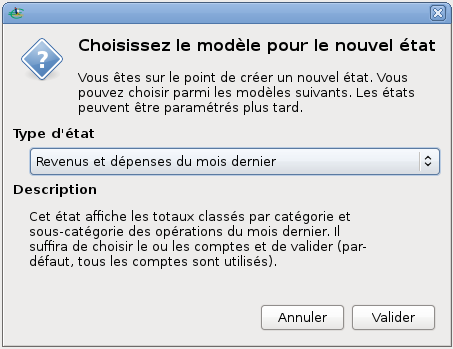
\includegraphics[scale=0.5]{image/screenshot/reportcreation_new}
\end{center}
\caption{Choix du modèle de l'état de départ}
\label{reportcreation-new-img}
\end{figure}
% image centrée
\fi

		\item sélectionnez \indexword{\menu{État vierge}}\index{etat@état !vierge} dans la liste déroulante ; par défaut, Grisbi ne sélectionne aucune donnée ; par votre sélection, vous ajouterez les données qui vous intéressent, et retirerez celles qui ne vous intéressent pas,
		\item validez : la fenêtre de création/modification des états s'affiche ; cet état porte par défaut le nom \menu{État vierge}, et vous pouvez lui donner un nouveau \indexword{nom}\index{etat@état !nommer} (voir la section \vref{reportscreation-display-general}, \menu{Généralités}),
    \end{enumerate}

% saut de page pour paragraphe solidaire
\newpage

 \item créer un état à partir d'un \indexword{état préformaté}\index{etat@état !préformaté} :
    \begin{enumerate}
		\item dans la barre d'outils, cliquez sur l'outil \menu{Nouvel état}, ou bien dans le panneau de navigation, cliquez-droit sur l'onglet \menu{Nouvel état} ou sur un quelconque de ses sous-onglets, et sélectionnez \menu{Nouvel état},
		\item une fenêtre s'affiche, contenant une liste déroulante et une zone de \ifIllustration description\refimage{reportcreation-new-img}, 
\else description,
\fi
		\item sélectionnez un des états préformatés, autre que \menu{État vierge} ou \menu{Recherche} (qui sert uniquement à rechercher des informations dans la base de données de Grisbi (voir la section \vref{search-advanced}, \menu{Recherche par états}),
		\item validez : la fenêtre de création/modification des états s'affiche ; cet état porte par défaut le nom de l'état préformaté, et vous pouvez lui donner un nouveau \indexword{nom}\index{etat@état !nommer} (voir la section \vref{reportscreation-display-general}, \menu{Généralités}) ,
    \end{enumerate}

 \item créer un état à partir d'un \indexword{état préexistant}\index{etat@état !préexistant} :
    \begin{enumerate}
		\item sélectionnez un état préexistant dans le panneau de navigation ou la barre d'information,
		\item cliquez sur l'outil \menu{Propriétés} dans la barre d'outils,
		\item la fenêtre de création/modification des états s'affiche ; la première chose que vous devrez faire sera de lui donner un nouveau \indexword{nom}\index{etat@état !nommer} pour ne pas seulement modifier l'état préexistant (voir la section \vref{reportscreation-display-general}, \menu{Généralités}). 
    \end{enumerate}
\end{itemize}


\section{Sélection des données\label{reportscreation-selection}}


La fenêtre de création/modification des états s'affiche, et vous pouvez en changer la taille et la position. Cette fenêtre comprend deux \ifIllustration panneaux verticaux\refimage{reportcreation-datas-img} :
\else panneaux verticaux :
\fi

\ifIllustration
% image centrée
\begin{figure}[htbp]
\begin{center}
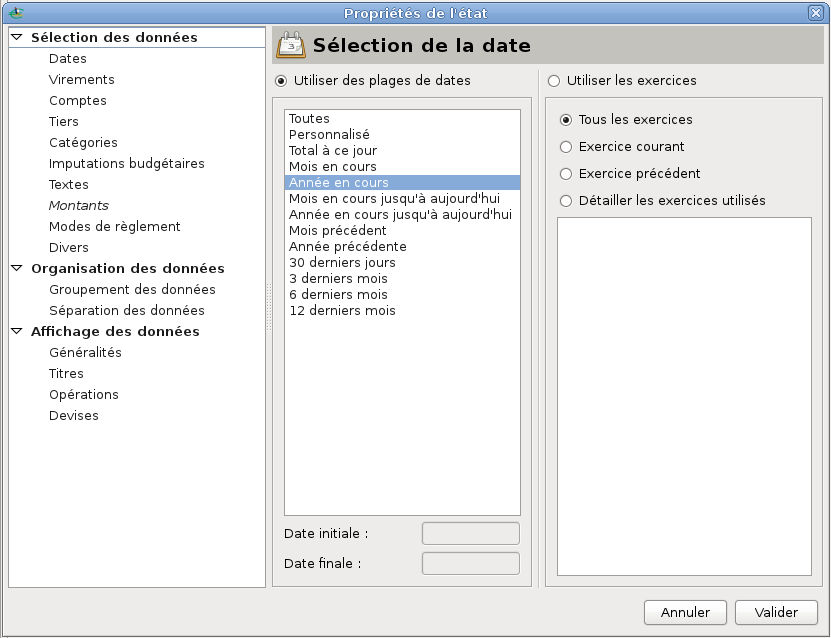
\includegraphics[scale=0.50]{image/screenshot/reportcreation_datas}
\end{center}
\caption{Fenêtre de création/modification des états}
\label{reportcreation-datas-img}
\end{figure}
% image centrée
\fi

\begin{itemize}
	 \item le panneau de gauche liste les trois grandes étapes de création d'un état : sélection, organisation et affichage des données ; chacune de ces étapes comprend une sous-liste que vous pouvez enrouler ou dérouler en cliquant sur le petit triangle à gauche du nom de l'étape ;

	\textbf{Note} : ces triangles peuvent être remplacés, en fonction du thème de l'environnement de bureau ou du gestionnaire de fenêtres que vous utilisez, par d'autres caractères tels que +, -, >, <, etc.
	 \item le panneau de droite affiche comme titre le critère sélectionné dans les sous-listes, et son contenu, c'est-à-dire les différentes sélections possibles.
\end{itemize}

Vous pouvez sélectionner un autre onglet en cliquant sur son nom, ou en naviguant dans le panneau des onglets avec les touches du clavier \key{Tabulation},  \key{Flèche Haut}, \key{Flèche Bas}, \key{Flèche Gauche}, \key{Flèche Droit}, \key{Page Haut}, \key{Page Bas}.
 
% espace pour lignes solidaires
\vspacepdf{5mm}         
Vous pouvez sélectionner vos données selon les critères suivants :

\begin{itemize}
	\item la date ou l'exercice ;
	\item le fait que l'opération soit ou non un virement et le type
	de virement ;
	\item le compte dans lequel l'opération est enregistrée ;
	\item le tiers ;
	\item la (sous-) catégorie ;
	\item la (sous-) imputation budgétaire ;
	\item du texte, pouvant se trouver dans :
		\begin{itemize}
			  \item des tiers (y compris sur une partie du nom),
			  \item les informations de tiers,
			  \item des (sous-) catégories (y compris sur une partie du nom),
			  \item des (sous-) imputations budgétaires (y compris sur une partie du nom),
			  \item des remarques,
			  \item des informations bancaires,
			  \item des pièces comptables,
			  \item des numéros de chèque ou de virement,
			  \item des numéros de rapprochement ;
		\end{itemize} 
	\item le montant ;
	\item le mode de règlement ;
	\item divers : le fait qu'une opération soit rapprochée ou non et qu'elle soit ventilée ou non.
\end{itemize}

% espace pour changement de thème
\vspacepdf{5mm}
La fenêtre de création/modification possède donc autant d'onglets que la liste ci-dessus possède d'items. Par défaut, Grisbi considère que vous désirez utiliser toutes les opérations de votre fichier de comptes. Vous ne devez donc garder que les opérations qui vous intéressent, en excluant les autres ; la sélection finale sera obtenue après application de toutes les sélections ci-dessus. Il est donc conseillé de vérifer tous les critères de sélection de la fenêtre de création/modification avant de valider votre état, bien que vous puissiez reprendre la sélection par la suite.

% espace pour changement de thème
\vspacepdf{5mm}
Les sous-sections suivantes décrivent en détail toutes ces possibilités de sélection de données.


\subsection{Dates (ou exercices)\label{reportscreation-selection-dates}}

Vous pouvez sélectionner soit des plages de dates, soit des exercices si
vous en avez défini.


\subsubsection{Dates}

Le choix par défaut est \menu{Utiliser des plages de dates}. S'il a été changé, vous pouvez le resélectionner en cochant le bouton \menu{Utiliser des plages de dates}. 

Vous pouvez faire les sélections suivantes :
% espace avant image 5mm
\vspacepdf{3mm}
% pas de référence à l'illustration car erreur de numéro de figure avec picins.
\begin{itemize}
	% image entourée par une liste (picins)
	\ifIllustration
	% supprimé car en html les figures entourées ne sont pas numérotées, et la numérotation des figures centrées décalée par rapport au pdf
	%\piccaption{Sélection de date}
	\label{reportcreation-datas-dates-img}
	\parpic[r]{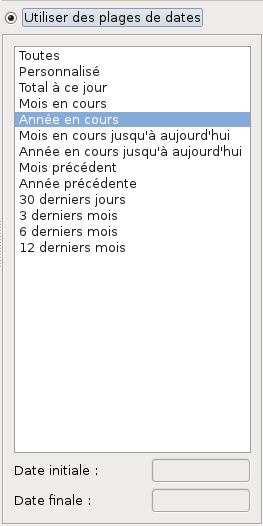
\includegraphics[scale=0.5]{image/screenshot/reportcreation_datas_dates}}
	\fi
	% image entourée par une liste (picins)
	\item \menu{Toutes} : toutes les dates ;
	\item \menu{Personnalisé} : une plage de dates personnalisée ; les zones de saisie des dates initiale et finale situées dans le bas du panneau deviennent actives ;
	\item des plages de dates prédéfinies qui vous permettent d'avoir un état valable en permanence sans être obligé de ressaisir à chaque fois les dates initiale et finale. Ces plages sont : 
	    \begin{itemize}
		\item \menu{Total à ce jour},
		\item \menu{Mois en cours},
		\item \menu{Année en cours},
		\item \menu{Mois en cours jusqu'à aujourd'hui},
		\item \menu{Année en cours jusqu'à aujourd'hui},
		\item \menu{Mois précédent}, c'est la sélection par défaut,
		\item \menu{Année précédente},
		\item \menu{30 derniers jours},
		\item \menu{3 derniers mois},
		\item \menu{6 derniers mois},
		\item \menu{12 derniers mois}.
	    \end{itemize}
\end{itemize} 


\ifIllustration
% espace après légende 8mm
\vspacepdf{10mm}
\fi

Pour continuer vos sélections, passez à l'onglet suivant.

\ifIllustration
% espace après image entourée
\vspacehevea{7mm}
\fi


\subsubsection{Exercices}

Pour sélectionner vos opérations par exercice, cochez le bouton correspondant \menu{Utiliser les exercices} (voir aussi le chapitre \vref{financialyear}, \menu{Exercices}). Vous pouvez faire les sélections suivantes :
% espace avant image 5mm
\vspacepdf{3mm}

% pas de référence à l'illustration car erreur de numéro de figure avec picins.
\begin{itemize}
	% image entourée par un paragraphe ( picins)
	\ifIllustration
	% supprimé car en html les figures entourées ne sont pas numérotées, et la numérotation des figures centrées décalée par rapport au pdf
	%\piccaption{Sélection d'exercice}
	\label{reportcreation-datas-financialyear-img}
	\parpic[r]{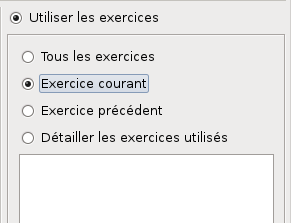
\includegraphics[scale=0.5]{image/screenshot/reportcreation_datas_financialyear}}
	\fi
	% image entourée par un paragraphe ( picins)
    \item \menu{Tous les exercices} ; ce choix est intéressant si vous décidez ensuite de séparer les opérations par exercices lors de l'affichage de l'état (voir la section \vref{reportscreation-organisation-separation}, \menu{Séparation des données}) ;
    \item \menu{Exercice courant} ;
    \item \menu{Exercice précédent} : ces deux choix vous permettent d'avoir des états qui seront toujours valables malgré les changements d'exercices ;
    \item \menu{Détailler les exercices utilisés} : sélectionnez ou désélectionnez un ou plusieurs des exercices définis dans votre fichier de comptes, en cliquant sur leur nom dans la liste juste en-dessous.
\end{itemize}

\ifIllustration
% espace après légende 14mm
\vspacepdf{9mm}
\else
% espace pour changement de thème
\vspacepdf{5mm}
\fi

Pour continuer vos sélections, passez à l'onglet suivant.

\ifIllustration
% espace après image entourée
\vspacehevea{2mm}
\fi


\subsection{Virements\label{reportscreation-selection-transfer}}

Vous choisissez ici la façon dont votre état traitera les opérations de virement. En cochant le bouton adéquat, vous pouvez \ifIllustration faire les sélections suivantes\refimage{reportcreation-datas-transfers-img} :
\else faire les sélections suivantes :
\fi

\ifIllustration
% image centrée
\begin{figure}[htbp]
\begin{center}
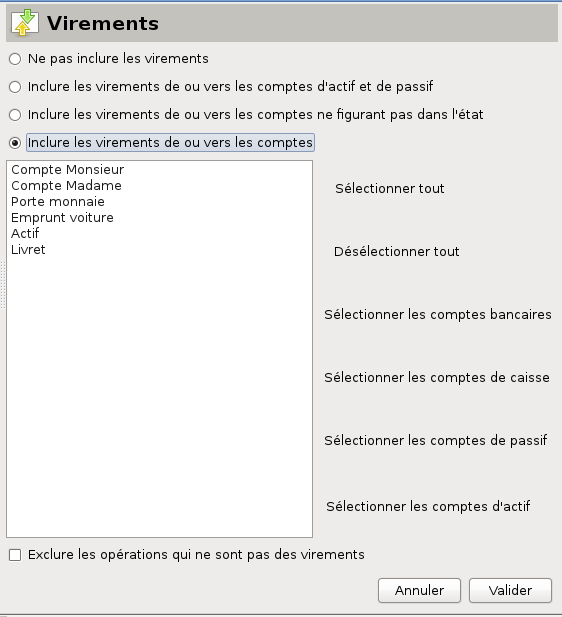
\includegraphics[scale=0.5]{image/screenshot/reportcreation_datas_transfers}
\end{center}
\caption{Sélection de virement}
\label{reportcreation-datas-transfers-img}
\end{figure}
% image centrée
\fi

\begin{itemize}
	\item \menu{Ne pas inclure les virements} : aucune des opérations de virement entre vos comptes ne sera incluse dans votre état ; cette option est intéressante si vous faites un état comportant tous les comptes ;
	\item \menu{Inclure les virements de ou vers les comptes d'actif et de passif} : ces comptes étant normalement utilisés pour vos créances et dettes (emprunts, prêts, etc.), il peut être intéressant de conserver ces virements dans votre état ;
	\item \menu{Inclure les virements de ou vers les comptes ne figurant pas dans l'état} : c'est le choix par défaut, il vous permet d'éliminer les virements entre comptes figurant dans l'état ;
	\item \menu{Inclure les virements de ou vers les comptes} : ceux que vous voulez conserver dans l'état ; ceci active la liste des comptes de votre fichier juste en-dessous, ainsi que les libellés de sélection par type de compte dans la partie droite du panneau : sélectionnez les comptes pour lesquels vous souhaitez conserver les virements, en cliquant sur leur nom dans la liste (la sélection multiple avec \key{Ctrl}\key{Clic} ou  \key{Majuscule}\key{Clic} est possible), ou en cliquant sur les libellés, qui vous permettent de choisir :
	
	\begin{itemize}
		  \item \menu{Sélectionner tout},
		  \item \menu{Désélectionner tout},
		  \item \menu{Sélectionner les comptes bancaires},
		  \item \menu{Sélectionner les comptes de caisse},
		  \item \menu{Sélectionner les comptes de passif},
		  \item \menu{Sélectionner les comptes d'actif} ;
	\end{itemize} 
	
	\item \menu{Exclure les opérations qui ne sont pas des virements}. Ceci vous permet par exemple de vérifier que tous vos virements s'équilibrent (le solde de l'état devra dans ce cas être égal à zéro).
\end{itemize} 

% espace pour changement de thème
\vspacepdf{5mm}
Pour continuer vos sélections, passez à l'onglet suivant.


\subsection{Comptes\label{reportscreation-selection-accounts}}

Pour sélectionner vos opérations en fonction des comptes où elles ont été enregistrées, cochez la case \menu{Sélectionner les opérations uniquement sur certains comptes}, qui par défaut \ifIllustration ne l'est pas\refimage{reportcreation-datas-accounts-img}.
% image centrée
\begin{figure}[htbp]
\begin{center}
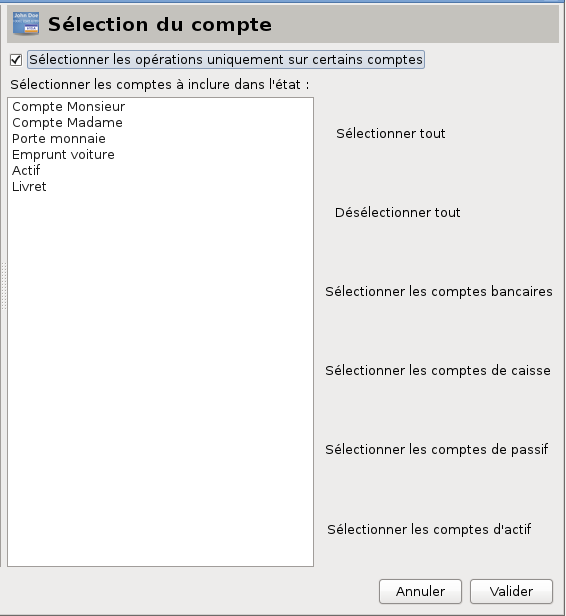
\includegraphics[scale=0.5]{image/screenshot/reportcreation_datas_accounts}
\end{center}
\caption{Sélection de compte}
\label{reportcreation-datas-accounts-img}
\end{figure}
% image centrée
\else ne l'est pas.
\fi

Ceci active la liste des comptes de votre fichier juste en-dessous, ainsi que les libellés de sélection par type de compte dans la partie droite du panneau ; sélectionnez les comptes désirés, en cliquant sur leur nom dans la liste (la sélection multiple avec \key{Ctrl}\key{Clic} ou  \key{Majuscule}\key{Clic} est possible), ou en cliquant sur les libellés, qui vous permettent de choisir :

\begin{itemize}
	  \item \menu{Sélectionner tout} ;
	  \item \menu{Désélectionner tout} ;
	  \item \menu{Sélectionner les comptes bancaires} ;
	  \item \menu{Sélectionner les comptes de caisse} ;
	  \item \menu{Sélectionner les comptes de passif} ;
	  \item \menu{Sélectionner les comptes d'actif}.
\end{itemize}

% espace pour changement de thème
\vspacepdf{5mm}
Pour continuer vos sélections, passez à l'onglet suivant.


\subsection{Tiers\label{reportscreation-selection-thirdparties}}

Pour sélectionner vos opérations en fonction des tiers avec lesquels elles ont été enregistrées, cochez la case \menu{Détailler les tiers}, qui par défaut \ifIllustration ne l'est pas\refimage{reportcreation-datas-thirdparts-img}.
% image centrée
\begin{figure}[htbp]
\begin{center}
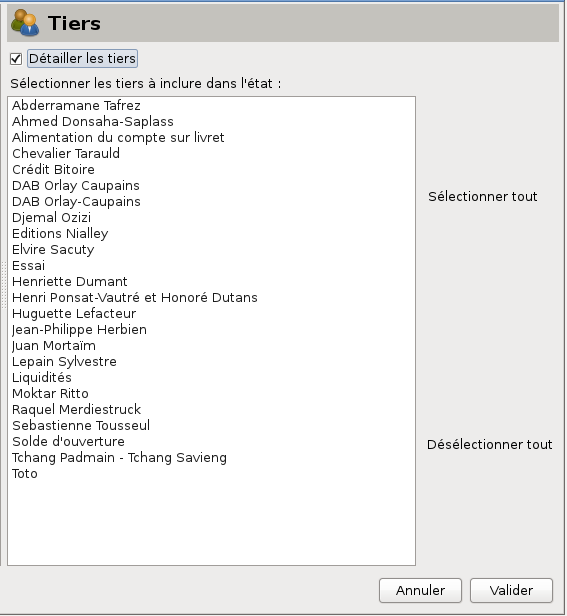
\includegraphics[scale=0.5]{image/screenshot/reportcreation_datas_thirdparts}
\end{center}
\caption{Sélection de tiers}
\label{reportcreation-datas-thirdparts-img}
\end{figure}
% image centrée
\else ne l'est pas.
\fi

Ceci active la liste des tiers de votre fichier juste en-dessous, ainsi que les libellés de sélection dans la partie droite du panneau ; sélectionnez les tiers désirés, en cliquant sur leur nom (la sélection multiple avec \key{Ctrl}\key{Clic} ou  \key{Majuscule}\key{Clic} est possible), ou en cliquant sur les libellés, qui vous permettent de choisir :

\begin{itemize}
	  \item \menu{Sélectionner tout} ;
	  \item \menu{Désélectionner tout}.
\end{itemize}

% espace pour changement de thème
\vspacepdf{5mm}
Pour continuer vos sélections, passez à l'onglet suivant.


\subsection{Catégories\label{reportscreation-selection-categories}}

Pour sélectionner vos opérations en fonction des catégories avec lesquelles elles ont été enregistrées, cochez la case \menu{Détailler les catégories utilisées}, qui par défaut \ifIllustration ne l'est pas\refimage{reportcreation-datas-categories-img}.
\else ne l'est pas.
\fi

\ifIllustration
% image centrée
\begin{figure}[htbp]
\begin{center}
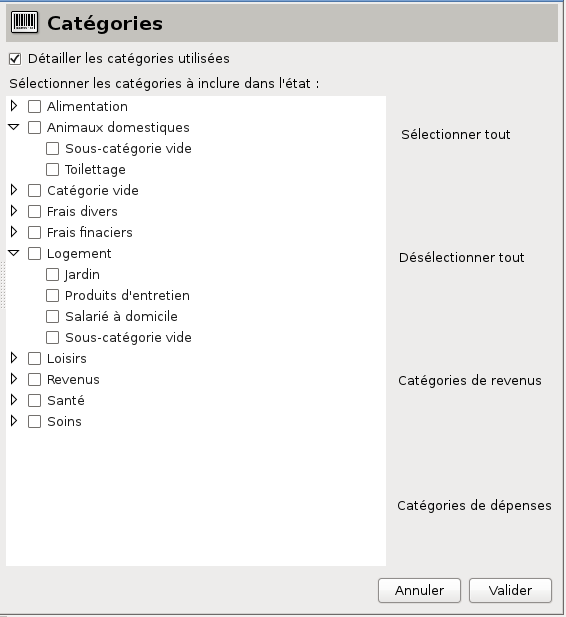
\includegraphics[scale=0.5]{image/screenshot/reportcreation_datas_categories}
\end{center}
\caption{Sélection de catégorie}
\label{reportcreation-datas-categories-img}
\end{figure}
% image centrée
\fi

Ceci active la liste des catégories de votre fichier juste en-dessous, ainsi que les libellés de sélection dans la partie droite du panneau ; vous pouvez (dés)afficher les sous-catégories en cliquant sur le petit triangle à gauche du nom de la catégorie.

\textbf{Note} : ces triangles peuvent être remplacés, en fonction du thème de l'environnement de bureau ou du gestionnaire de fenêtres que vous utilisez, par d'autres caractères tels que +, -, >, <, etc. 

Sélectionnez  les (sous-) catégories, individuellement en cliquant sur leur case à gauche, ou en cliquant sur les libellés, qui vous permettent de choisir :

\begin{itemize}
	  \item \menu{Sélectionner tout} ;
	  \item \menu{Désélectionner tout} ;
	  \item \menu{Catégories de revenus} ;
	  \item \menu{Catégories de dépenses}.
\end{itemize}

% espace pour changement de thème
\vspacepdf{5mm}

Pour continuer vos sélections, passez à l'onglet suivant.


\subsection{Imputations budgétaires\label{reportscreation-selection-budgetarylines}}

Cela fonctionne exactement comme pour le critère \menu{Catégories}.

Pour sélectionner vos opérations en fonction des imputations budgétaires avec lesquelles elles ont été enregistrées, cochez la case \menu{Détailler les imputations budgétaires utilisées}, qui par défaut \ifIllustration ne l'est pas\refimage{reportcreation-datas-budgetlines-img}.
% image centrée
\begin{figure}[htbp]
\begin{center}
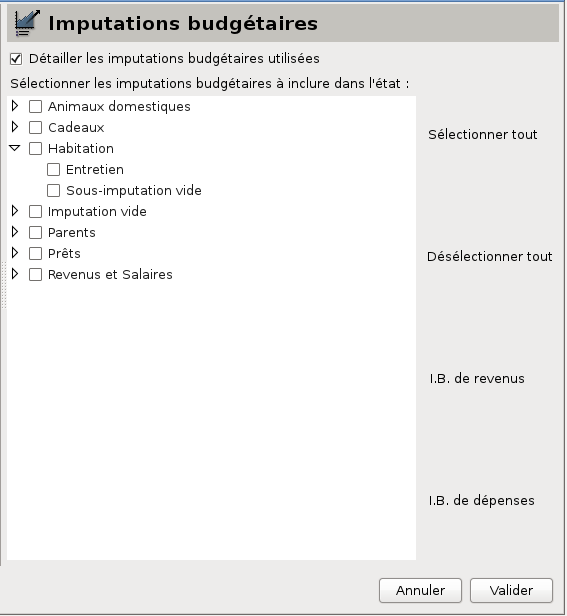
\includegraphics[scale=0.5]{image/screenshot/reportcreation_datas_budgetlines}
\end{center}
\caption{Sélection d'imputation budgétaire}
\label{reportcreation-datas-budgetlines-img}
\end{figure}
% image centrée
\else ne l'est pas.
\fi

Ceci active la liste des imputations budgétaires juste en-dessous, ainsi que les libellés de sélection dans la partie droite du panneau ; vous pouvez (dés)afficher les sous-imputations budgétaires en cliquant sur le petit triangle à gauche du nom de l'imputation.

\textbf{Note} : ces triangles peuvent être remplacés, en fonction du thème de l'environnement de bureau ou du gestionnaire de fenêtres que vous utilisez, par d'autres caractères tels que +, -, >, <, etc.

Sélectionnez les (sous-) imputations budgétaires, individuellement en cliquant sur leur case à gauche, ou en cliquant sur les libellés, qui vous permettent de choisir :

\begin{itemize}
	\item \menu{Sélectionner tout} ;
	\item \menu{Désélectionner tout} ;
	\item \menu{Imputation budgétaire de revenus} ;
	\item \menu{Imputation budgétaire de dépenses}.
\end{itemize}

% espace pour changement de thème
\vspacepdf{5mm}
Pour continuer vos sélections, passez à l'onglet suivant.


\subsection{Textes\label{reportscreation-selection-text}}

\textbf{Note} : il se peut que la fenêtre de création/modification des états n'affiche  pas entièrement le panneau droit de sélection de texte : il vous faudra alors agrandir manuellement sa taille.
% espace après Attention ou Note  : 5 mm
\vspacepdf{5mm}

Vous pouvez faire des sélections complexes basées sur le contenu (texte ou nombre) enregistré dans les champs d'une opération. Il s'agit de comparer le contenu du champ sélectionné à une valeur à travers un opérateur, et ceci pour toutes les opérations de votre fichier de comptes, tout au moins celles qui ont déjà été sélectionnées par les autres sélections de votre état en cours de création.

% espace pour changement de thème
\vspacepdf{5mm}
Créer une sélection d'après les \menu{Textes} consiste donc à définir une  phrase simple du type sujet-verbe-complément, et plus précisément ici, une instruction \og champ-opérateur-valeur \fg{}. Les opérateurs sont soit \indexword{alphanumériques}\index{opérateur !alphanumérique} s'il vous faut comparer des textes, soit \indexword{numériques}\index{opérateur !numérique} pour comparer des nombres. 

% espace pour changement de thème
\vspacepdf{5mm}
Pour sélectionner vos opérations en fonction de certains contenus enregistrés dans leurs champs, cochez la case \menu{Sélectionner les opérations d'après leur contenu}, qui par défaut \ifIllustration ne l'est pas\refimage{reportcreation-datas-text-img}.
\else ne l'est pas. \fi Ceci active les champs de définition de la phrase, qui s'affiche par défaut sur trois lignes juste en-dessous.

\ifIllustration
% image centrée
\begin{figure}[htbp]
\begin{center}
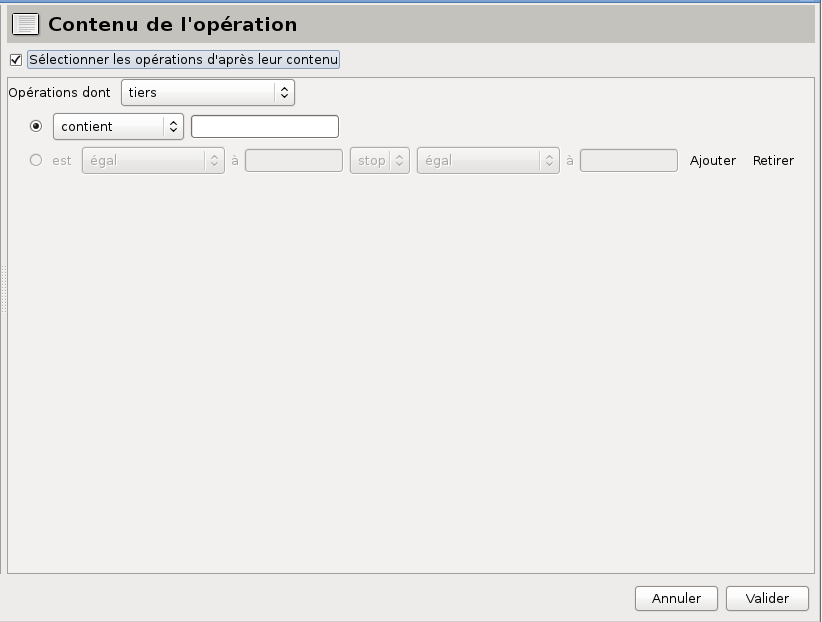
\includegraphics[scale=0.5]{image/screenshot/reportcreation_datas_text}
\end{center}
\caption{Sélection de texte}
\label{reportcreation-datas-text-img}
\end{figure}
% image centrée
\fi

% espace pour changement de thème
\vspacepdf{5mm}
La 1\up{re} ligne sert à définir le champ. Les champs disponibles sont :

\begin{itemize}
	    \item \menu{tiers} ;
	    \item \menu{information du tiers} ;
	    \item \menu{catégorie} ;
	    \item \menu{sous-catégorie} ;
	    \item \menu{imputation budgétaire} ;
	    \item \menu{sous-imputation budgétaire} ;
	    \item \menu{remarque} ;
	    \item \menu{information bancaire} ;
	    \item \menu{pièce comptable} ;
	    \item \menu{\no chèque} ;
	    \item \menu{\no de rapprochement}.
\end{itemize}

La 2\up{e} ligne sert à définir l'opérateur à appliquer et la valeur si le contenu du champ est un texte. 

Les \indexword{opérateurs alphanumériques}\index{opérateur !alphanumérique} disponibles sont :

\begin{itemize}
	\item \menu{contient} ;
	\item \menu{ne contient pas} ;
	\item \menu{commence par} ;
	\item \menu{se termine par} ;
	\item \menu{est vide} ;
	\item \menu{est non vide}.
\end{itemize}

La 3\up{e} ligne sert à définir l'opérateur à appliquer et la valeur si le contenu du champ est un nombre. 

Les \indexword{opérateurs numériques}\index{opérateur !numérique} disponibles sont :

\begin{itemize}
	\item \menu{égal} ;
	\item\menu{inférieur} ;
	\item \menu{inférieur ou égal} ;
	\item \menu{supérieur} ;
	\item\menu{supérieur ou égal} ;
	\item\menu{différent de} ;
	\item \menu{le plus grand}.
\end{itemize}

De plus, la 3\up{e} ligne permet de faire une double comparaison de façon à pouvoir, par exemple, sélectionner les contenus supérieurs à une valeur donnée, sauf les contenus égaux à une autre valeur. Pour cela, un opérateur concatène deux instructions \og champ-opérateur-valeur \fg{}. 

Les \indexword{opérateurs de concaténation}\index{opérateur !concaténation} sont :

\begin{itemize}
	\item \menu{et} ;
	\item \menu{ou} ;
	\item \menu{sauf} ;
	\item \menu{stop} (qui est le choix par défaut, et qui signifie qu'il n'y a pas d'autre
	critère à appliquer).
\end{itemize}

% espace pour changement de thème
\vspacepdf{5mm}
Ces trois lignes permettent de définir une instruction de deux manières différentes :
\begin{enumerate}
	 \item si le contenu du champ est un texte, l'instruction sera du type \og champ-opérateur alphanumérique-texte \fg{} (utilisation des seules lignes 1 et 2) ;
	 \item si le contenu du champ est un nombre, l'instruction sera du type \og champ-opérateur numérique-texte \fg{} \og opérateur de concaténation \fg{} \og opérateur numérique-texte \fg{} (utilisation des seules lignes 1 et 3).
\end{enumerate}

Tous les contenus des champs contenant du texte sont considérés comme du texte, à l'exception des champs \menu{\no chèque}, \menu{pièce comptable} et \menu{\no de rapprochement}, qui peuvent être considérés soit comme du texte, soit comme des nombres, car ils sont enregistrés comme tels dans votre fichier de comptes. En effet, d'une part leur signification n'est pas purement numérique (vous ne chercherez jamais à les additionner ou les multiplier, n'est-ce pas ?), d'autre part, il n'est pas impossible qu'ils puissent contenir des lettres. Par exemple, le champ \menu{tiers} (un nom est un texte) autorisera donc seulement le premier type d'instruction, tandis que le champ \menu{\no chèque}, \menu{pièce comptable} ou \menu{rapprochement bancaire} autoriseront le premier et le deuxième type d'instruction, que vous choisirez selon votre besoin ;  dans les deux cas, la ligne d'instruction non utilisée restera en grisé.

% espace pour changement de thème
\vspacepdf{5mm}
En pratique, pour créer une instruction, procédez comme suit :

\begin{enumerate}
	 \item dans la 1\up{re} ligne, choisissez, à droite de \menu{Opérations dont}, le champ dans la liste déroulante commençant par \menu{tiers} ; 
	 \item si le choix de la 2\up{e} ou 3\up{e} ligne vous est laissé, cliquez sur le bouton à gauche de l'une d'elles, en fonction de ce que vous voulez sélectionner ; celle qui n'est pas choisie s'affiche en grisé ; 
	 \item si la 2\up{e} ligne est validée :
		\begin{enumerate}
			    \item choisissez l'opérateur dans la liste déroulante commençant par \menu{contient},
			    \item saisissez, dans la zone à droite de la liste, le texte que vous recherchez dans vos opérations ;
		\end{enumerate}	
	 \item  si la 3\up{e} ligne est validée : 	
		\begin{enumerate}
			    \item choisissez, à droite de  \menu{est}, l'opérateur dans la première liste déroulante commençant par \menu{égal},
			    \item saisissez, dans la zone à droite de \menu{à}, le nombre que vous voulez comparer dans vos opérations,
			    \item l'instruction est terminée si vous laissez \menu{stop} dans la deuxième liste déroulante commençant par \menu{et} ; si vous faites un autre choix que \menu{stop} dans cette deuxième liste, la suite de l'instruction est validée et vous pouvez compléter l'instruction,
			    \item choisissez alors, à droite, l'opérateur dans la troisième liste déroulante commençant par \menu{égal},
			    \item saisissez, dans le champ à droite de \menu{à}, le nombre que vous  vous voulez comparer dans vos opérations ;
		\end{enumerate}	
	 \item l'instruction est terminée.
\end{enumerate}

Si vous voulez affiner votre sélection, vous pouvez encore créer une ou
plusieurs autres instructions, qui seront liées aux précédentes par des opérateurs de concaténation : ceux-ci sont les mêmes que ci-dessus, excepté le \menu{stop} qui n'a pas de raison d'être ici, puisqu'il s'agit de continuer. 

% espace pour changement de thème
\vspacepdf{5mm}
Pour ajouter une instruction supplémentaire, procédez \ifIllustration comme suit\refimage{reportcreation-datas-multiplesText-img} :
% image centrée
\begin{figure}[htbp]
\begin{center}
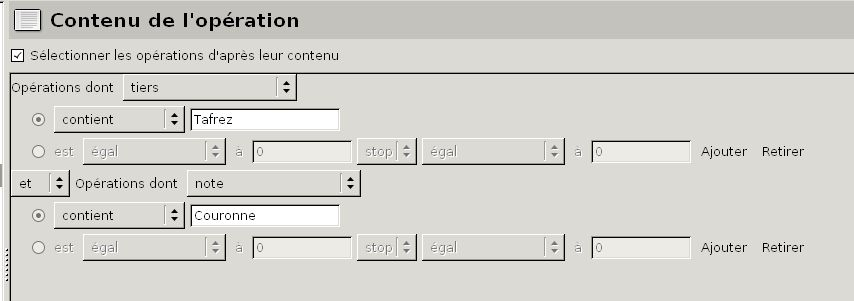
\includegraphics[scale=0.5]{image/screenshot/reportcreation_datas_multiplesText}
\end{center}
\caption{Sélection multiple de texte}
\label{reportcreation-datas-multiplesText-img}
\end{figure}
% image centrée
\else comme suit :
\fi

\begin{itemize}
	\item à la fin de la 3\up{e} ligne d'une instruction, à droite, cliquez sur le libellé \menu{Ajouter} ;
	 \item trois nouvelles lignes s'affichent pour définir votre nouvelle instruction ; elles sont identiques aux lignes de la première instruction, sauf que la 1\up{re} ligne commence par une liste déroulante commençant par \menu{et} ;
	 \item choisissez l'opérateur de concaténation ( \menu{et},  \menu{ou},  \menu{sauf}) qui vous convient pour ajouter votre nouvelle instruction ;
	 \item définissez cette nouvelle instruction comme vous l'avez fait pour la première.
\end{itemize}

% espace pour changement de thème
\vspacepdf{5mm}
Pour supprimer une instruction, cliquez sur le libellé \menu{Retirer} à la fin de
sa 3\up{e} ligne.

% espace pour changement de thème
\vspacepdf{5mm}
Pour continuer vos sélections, passez à l'onglet suivant.

\ifIllustration
% saut de page pour titre solidaire
\newpage
\fi


\subsection{Montants\label{reportscreation-selection-amount}}

La sélection d'après les \menu{Montants} fonctionne de manière semblable à celle des \menu{Textes}, mais elle est plus simple car il ne s'agit ici que de nombres, sans texte.

% espace avant Attention ou Note  : 5 mm
\vspacepdf{5mm}
\textbf{Note} : il se peut que la fenêtre de création/modification des états n'affiche  pas entièrement le panneau droit de sélection de texte : il vous faudra alors agrandir manuellement sa taille.

% espace après Attention ou Note  : 5 mm
\vspacepdf{5mm}
Vous pouvez faire des sélections complexes basées sur le nombre enregistré dans les champs d'une opération. Il s'agit de comparer le contenu du champ sélectionné à une valeur à travers un opérateur, et ceci pour toutes les opérations de votre fichier de comptes, tout au moins celles qui ont déjà été sélectionnées par les autres sélections de votre état en cours de création.

% espace pour changement de thème
\vspacepdf{5mm}
Créer une sélection consiste donc à définir une  phrase simple du type sujet-verbe-complément, et plus précisément ici, une instruction \og champ-opérateur-valeur \fg{}. Les opérateurs sont uniquement \indexword{numériques}\index{opérateur !numérique}, pour comparer des nombres. 

% espace pour changement de thème
\vspacepdf{5mm}
Pour sélectionner vos opérations en fonction de certains contenus enregistrés dans leurs champs, cochez la case \menu{Sélectionner les opérations d'après les montants}, qui par défaut \ifIllustration ne l'est pas\refimage{reportcreation-datas-amounts-img}. Ceci active les champs de définition de la phrase, qui s'affiche par défaut sur  une seule ligne juste en-dessous.

% image centrée
\begin{figure}[htbp]
\begin{center}
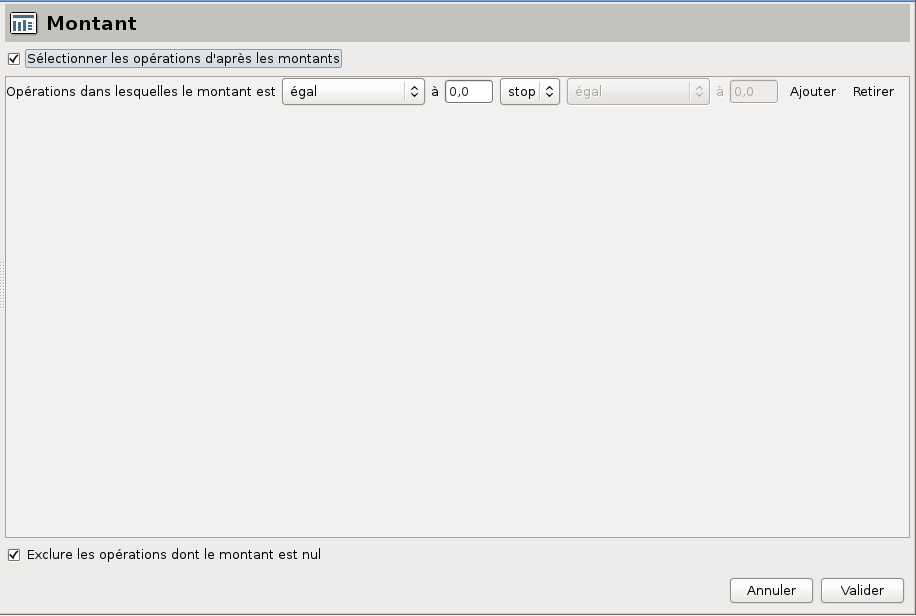
\includegraphics[scale=0.5]{image/screenshot/reportcreation_datas_amounts}
\end{center}
\caption{Sélection de montant}
\label{reportcreation-datas-amounts-img}
\end{figure}
% image centrée
\else ne l'est pas.
\fi

Cette ligne  sert à définir l'opérateur à appliquer et le nombre à comparer. Les \indexword{opérateurs numériques}\index{opérateur !numérique} disponibles sont :

\begin{itemize}
	\item \menu{égal} ;
	\item\menu{inférieur} ;
	\item \menu{inférieur ou égal} ;
	\item \menu{supérieur à} ;
	\item\menu{supérieur ou égal} ;
	\item\menu{différent de} ;
	\item \menu{nul} ;
	\item \menu{non nul} ;
	\item \menu{positif} ;
	\item \menu{négatif}.
\end{itemize}

De plus, elle permet de faire une double comparaison, de façon à pouvoir, par exemple, sélectionner les contenus supérieurs à une valeur donnée, sauf les contenus égaux à une autre valeur. Pour cela, un deuxième opérateur concatène deux instructions \og champ-opérateur-valeur \fg{}. 

Les \indexword{opérateurs de concaténation}\index{opérateur !concaténation} sont :

\begin{itemize}
	\item \menu{et} ;
	\item \menu{ou} ;
	\item \menu{sauf} ;
	\item \menu{stop} (qui est le choix par défaut, et qui signifie qu'il n'y a pas d'autre critère à appliquer).
\end{itemize}


Cette ligne permet de définir l'instruction de la manière suivante : elle sera du type \og champ-opérateur numérique-texte \fg{} \og opérateur de concaténation \fg{} \og opérateur numérique-texte \fg{}.

%ATTENTION , LA PARTIE APRÈS L'OPÉRATEUR DE CONCATÉNATION N'EST JAMAIS VALIDÉE  : Il s'agit d'un bogue connu.

% espace avant Attention ou Note  : 5 mm
\vspacepdf{5mm}
\textbf{Note} : les dépenses sont des montants négatifs  ; ces montants doivent donc être précédés du signe \og \textbf{-} \fg{} (moins) dans les champs où vous saisissez des montants négatifs, par exemple -72,15.

% espace avant Attention ou Note  : 5 mm
\vspacepdf{5mm}
\textbf{Note} : Grisbi ne fera pas de contrôle de cohérence sur vos critères. Par exemple, si vous voulez sélectionner les opérations \og dont le numéro de relevé est supérieur ou égal à 20 sauf celles dont le numéro de relevé est supérieur ou égal à 5 \fg{}, vous obtiendrez un état vide, tout simplement. L'erreur peut être difficile à déceler, et on n'est jamais trop fort pour ce calcul !
% espace arès Attention ou Note  : 5 mm
\vspacepdf{5mm}

En pratique, pour créer une instruction, procédez comme suit :

\begin{enumerate}
	\item dans l'unique ligne, choisissez, à droite de \menu{Opérations dans lesquelles le montant est}, le champ dans la liste déroulante commençant par \menu{égal} ; 
	\item saisissez, dans la zone à droite de \menu{à}, le nombre que vous voulez comparer dans vos opérations ;
	\item  l'instruction est terminée si vous laissez \menu{stop} dans la deuxième liste déroulante commençant par \menu{et} ; si vous faites un autre choix que \menu{stop} dans cette deuxième liste, la suite de l'instruction est validée et vous pouvez compléter l'instruction ;
	 \item choisissez alors, à droite, l'opérateur dans la troisième liste déroulante commençant par \menu{égal} ;
	\item saisissez, dans le champ à droite de \menu{à}, le nombre que vous voulez comparer dans vos opérations ;
	\item l'instruction est terminée.
\end{enumerate}

Si vous voulez affiner votre sélection, vous pouvez ajouter une ou
plusieurs autres instructions, qui seront liées aux précédentes par des opérateurs de concaténation : ceux-ci sont les mêmes que ci-dessus, excepté le \menu{stop} qui n'a pas de raison d'être ici, puisqu'il s'agit de continuer. Pour créer une instruction supplémentaire, procédez \ifIllustration comme suit\refimage{reportcreation-datas-multiplesAmounts-img} :

% image centrée
\begin{figure}[ht]
\begin{center}
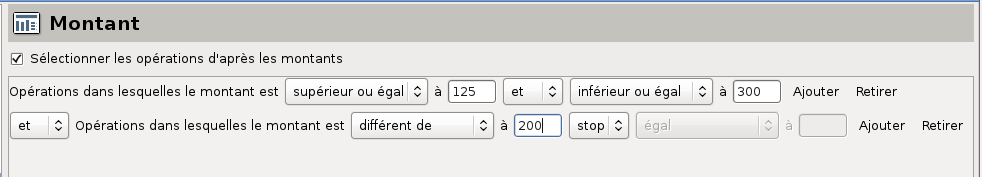
\includegraphics[scale=0.5]{image/screenshot/reportcreation_datas_multiplesAmounts}
\end{center}
\caption{Sélection multiple de montant}
\label{reportcreation-datas-multiplesAmounts-img}
\end{figure}
% image centrée
\else comme suit :
\fi

\begin{itemize}
	 \item cliquez sur le libellé \menu{Ajouter} ;
	 \item une nouvelle ligne s'affiche pour définir votre nouvelle instruction ; elle est identique aux lignes de la première instruction, sauf que la 1\up{re} ligne commence par une liste déroulante commençant par \menu{et} ;
	 \item choisissez l'opérateur de concaténation ( \menu{et},  \menu{ou},  \menu{sauf}) qui vous convient pour ajouter votre nouvelle instruction ;
	 \item définissez cette nouvelle instruction comme vous l'avez fait pour la première.
\end{itemize}

% espace pour changement de thème
\vspacepdf{5mm}
Pour supprimer une instruction, cliquez sur le libellé \menu{Retirer} à la fin de sa ligne.

% espace pour changement de thème
\vspacepdf{5mm}

Pour continuer vos sélections, passez à l'onglet suivant.


\subsection{Modes de règlement\label{reportscreation-selection-paiementmode}}

Pour sélectionner vos opérations en fonction du mode de règlement, cochez la case  \menu{Sélectionner les opérations en fonction des modes de règlement}, qui par défaut 
\ifIllustration ne l'est pas\refimage{reportcreation-datas-modes-img}.
\else ne l'est pas.
\fi

\ifIllustration
% image centrée
\begin{figure}[h!]
\begin{center}
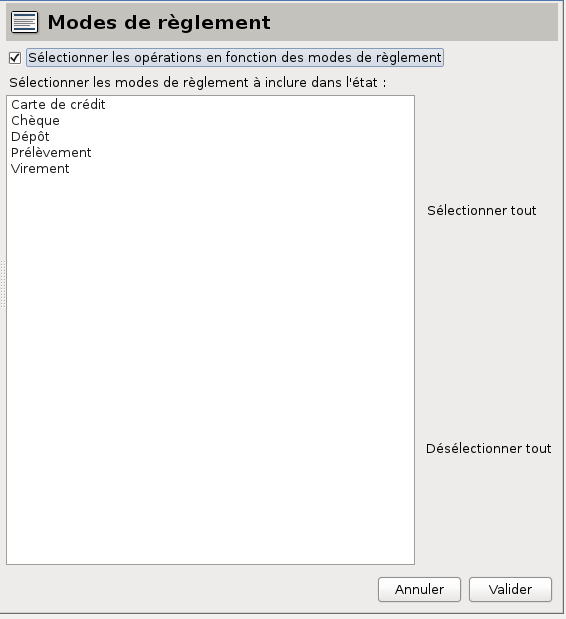
\includegraphics[scale=0.5]{image/screenshot/reportcreation_datas_modes}
\end{center}
\caption{Sélection des mode de règlement}
\label{reportcreation-datas-modes-img}
\end{figure}
% image centrée
\fi

Ceci active la liste des modes de règlement de votre fichier juste en-dessous, ainsi que les libellés de sélection dans la partie droite du panneau ; sélectionnez les modes de règlement désirés, en cliquant sur leur nom (la sélection multiple avec \key{Ctrl}\key{Clic} ou  \key{Majuscule}\key{Clic} est possible), ou en cliquant sur les libellés, qui vous permettent de choisir :

\begin{itemize}
	  \item \menu{Sélectionner tout} ;
	  \item \menu{Désélectionner tout}.
\end{itemize}

\ifIllustration
\else
% espace pour changement de thème
\vspacepdf{5mm}
\fi

Pour continuer vos sélections, passez à l'onglet suivant.


\subsection{Divers\label{reportscreation-selection-misc}}

Vous pouvez affiner votre sélection en ajoutant des critères sur les opérations rapprochées et \ifIllustration ventilées\refimage{reportcreation-datas-misc-img}.
\else ventilées.
\fi

\ifIllustration
% image centrée
\begin{figure}[htbp]
\begin{center}
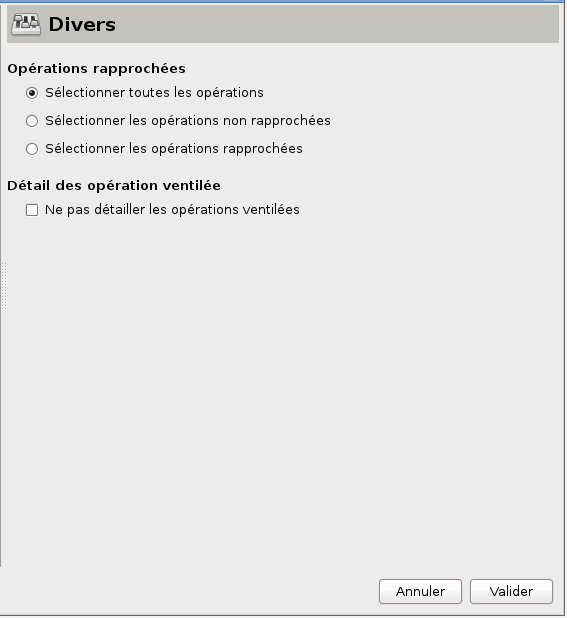
\includegraphics[scale=0.5]{image/screenshot/reportcreation_datas_misc}
\end{center}
\caption{Sélections diverses}
\label{reportcreation-datas-misc-img}
\end{figure}
% image centrée
\fi


\subsubsection{Opérations rapprochées}

En cochant le bouton adéquat, vous pouvez sélectionner :

\begin{itemize}
	\item \menu{toutes les opérations ; c'est le cas par défaut} ;
	\item \menu{les opérations non rapprochées uniquement} ;
	\item \menu{les opérations rapprochées uniquement}.
\end{itemize} 


\subsubsection{Détail des opérations ventilées}

En cochant le bouton, vous pouvez choisir de ne pas détailler les opérations ventilées. Par défaut la case n'est pas cochée.

\ifIllustration
\else
% espace pour changement de thème
\vspacepdf{5mm}
\fi

Vos sélections sont terminées. Pour organiser vos données, passez à l'onglet suivant.


\section{Organisation des données\label{reportscreation-organisation}}


Organiser les données de votre état signifie les grouper ou les séparer suivant vos besoins.


\subsection{Groupement des données\label{reportscreation-organisation-group}}

Cet onglet permet de grouper vos données selon  différents critères et \ifIllustration différents niveaux\refimage{reportcreation-organisation-grouping-img}.
% image centrée
\begin{figure}[htbp]
\begin{center}
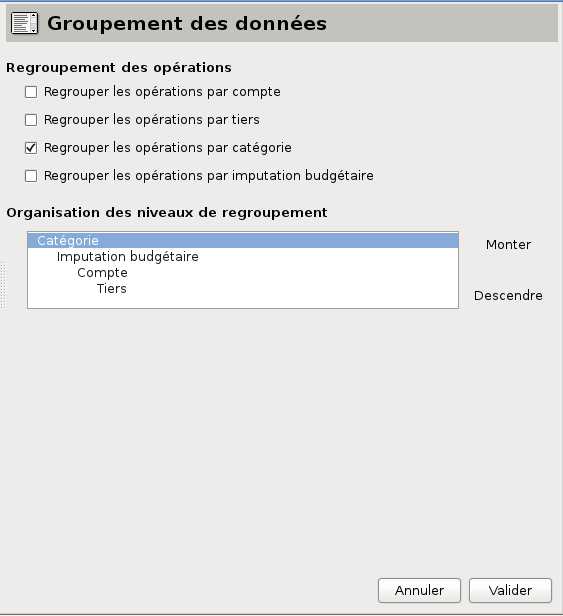
\includegraphics[scale=0.5]{image/screenshot/reportcreation_organisation_grouping}
\end{center}
\caption{Organisation des niveaux de regroupement}
\label{reportcreation-organisation-grouping-img}
\end{figure}
% image centrée
\else différents niveaux.
\fi


\subsubsection{Regroupement des opérations\label{reportscreation-organisation-group-operations}}

Sous ce libellé, définissez les \indexword{niveaux de regroupement}\index{niveau de regroupement} que vous voulez pour votre état, en cochant la case correspondante parmi les possibilités suivantes :

\begin{itemize}
	\item le compte ;
	\item le tiers ;
	\item la catégorie ; c'est le cas par défaut ;
	\item l'imputation budgétaire.
\end{itemize}

Il est rare qu'ils soient tous les quatre nécessaires, et il se peut tout à fait que vous désiriez n'en utiliser aucun. C'est votre choix. 


\subsubsection{Organisation des niveaux de regroupement\label{reportscreation-organisation-group-levels}}

Sous ce libellé, l'ordre par défaut des niveaux est indiqué dans un cadre. Si vous avez sélectionné les quatre niveaux en gardant l'ordre par défaut, vos opérations seront regroupées, au plus haut niveau, par catégories. À l'intérieur de chaque catégorie, les opérations seront regroupées par imputation budgétaire, à l'intérieur de chaque imputation budgétaire, par tiers, et enfin à l'intérieur de chaque tiers, par compte.

Ajustez cet ordre en sélectionnant  avec la souris le niveau à déplacer, puis cliquez sur les flèches \menu{Monter} ou \menu{Descendre} pour le placer à l'endroit voulu. Répétez l'opération autant de fois que nécessaire.

Seuls les niveaux sélectionnés dans \menu{{Regroupement des opérations}} doivent être correctement positionnés, et les autres ne seront pas concernés.

% espace pour changement de thème
\vspacepdf{5mm}
Pour continuer l'organisation de vos données, passez à l'onglet suivant.


\subsection{Séparation des données\label{reportscreation-organisation-separation}}

Vous pouvez choisir de séparer vos données en cochant les \ifIllustration cases suivantes\refimage{reportcreation-organisation-separation-img} :
\else cases suivantes :
\fi

\begin{itemize}
	\item \menu{Séparer  les revenus et les dépenses} ; par défaut, ils sont séparés ;
	\item \menu{Séparer les résultats par exercice} : ce choix n'est disponible que si vous avez choisi de sélectionner les opérations selon les exercices dans l'onglet \menu{Sélection/Dates} ;
	\item \menu{Séparer les résultats par période} : en cochant cette case, deux listes déroulantes sont validées :
		\begin{itemize}
			\item \menu{Période de temps} : vous avez le choix entre journée, semaine, mois et année ; choisissez la période voulue dans la liste,
			\item \menu{Début de la semaine} :  vous avez le choix entre tous les jours de la semaine ; choisissez le jour de départ de la période dans la liste.
		\end{itemize} 
\end{itemize} 

\ifIllustration
% image centrée
\begin{figure}[htbp]
\begin{center}
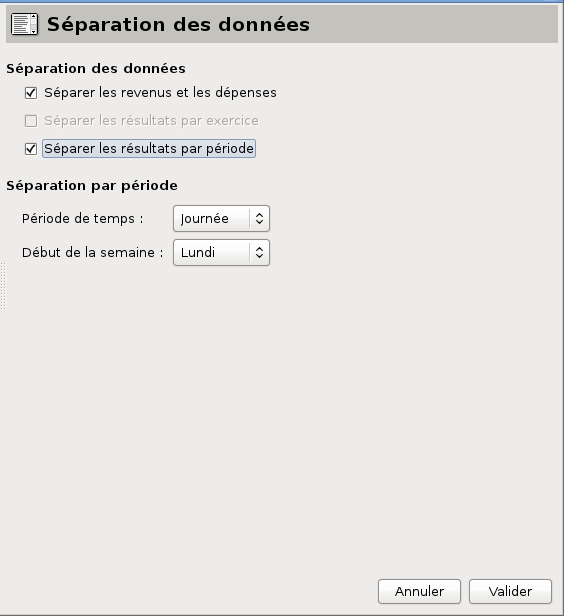
\includegraphics[scale=0.5]{image/screenshot/reportcreation_organisation_separation}
\end{center}
\caption{Séparation des données}
\label{reportcreation-organisation-separation-img}
\end{figure}
% image centrée
\fi

% espace pour changement de thème
\vspacepdf{5mm}
Pour configurer l'affichage de vos données, passez à l'onglet suivant.


\section{Affichage des données\label{reportscreation-display}}


Cet onglet vous permet de définir la façon dont les données de votre état, sélectionnées et
organisées dans les étapes précédentes, seront affichées. Il comprend quatre onglets :

\begin{itemize}
	\item \menu{Généralités} ;
	\item \menu{Titres} ;
	\item \menu{Opérations} ;
	\item \menu{Devises}.
\end{itemize} 


\subsection{Généralités\label{reportscreation-display-general}}

Dans cet onglet vous pouvez définir les paramètres \ifIllustration suivants\refimage{reportcreation-display-main-img} :
\else suivants :
\fi

\begin{itemize}
	\item  \menu{Nom de l'état}\index{etat@état !nommer} : saisissez son \indexword{nom}, il est à votre entière convenance ;
	\item  \menu{Afficher le nombre d'opérations avec les totaux} :  si vous cochez cette case, à chaque fois que l'état affichera un total ou un sous-total, il affichera à gauche de celui-ci et entre parenthèses le nombre d'opérations correspondantes ;	
	\item  \menu{Considérer les tiers de ce rapport comme un tiers virtuel} : si cette case est cochée, l'ensemble des tiers que vous avez éventuellement sélectionnés pour cet état forme un \indexword{\og tiers virtuel \fg{}} \index{tiers virtuel} ; ce tiers virtuel a pour nom le nom de l'état (voir le paragraphe \vref{reportscreation-display-general-virtualThird}, \menu{Tiers virtuel}). 
\end{itemize}

\ifIllustration
% image centrée
\begin{figure}[htbp]
\begin{center}
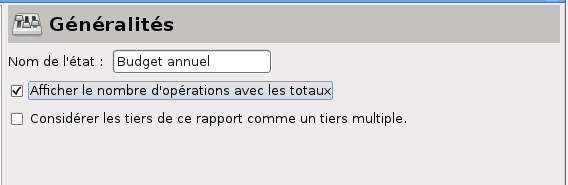
\includegraphics[scale=0.5]{image/screenshot/reportcreation_display_main} :
\end{center}
\caption{Affichage des généralités}
\label{reportcreation-display-main-img}
\end{figure}
% image centrée
\fi


\subsubsection{Tiers virtuel\label{reportscreation-display-general-virtualThird}}

Grisbi permet d'utiliser des tiers virtuels : un tiers virtuel est un \emph{état} qui représente une liste de plusieurs tiers.

Lorsque vous saisissez une opération avec pour tiers un tiers virtuel, Grisbi enregistre, au moment de sa validation, une opération identique (montant, catégorie, imputation budgétaire, moyen de paiement etc.) pour \emph{chacun} des tiers représentés par ce tiers virtuel. Par exemple, vous pouvez saisir en une seule fois un appel à cotisation pour 200 adhérents d'une association, ce qui représente un gain de temps très appréciable \ldots

%espace pour changement de thème
\vspacepdf{5mm}
La création d'un tiers virtuel est celle d'un état comprenant la liste de tous les tiers qui vous intéressent.

\ifIllustration
%espace pour changement de thème
\vspacepdf{5mm}
\fi

Pour \indexword{créer un tiers virtuel}\index{tiers virtuel !créer}, procédez comme suit :

\begin{enumerate}
	\item  commencez la procédure de création d'un état à la section \vref{reportscreation-start} ; \menu{Choix du modèle de l'état de départ} ; 
	\item quand la fenêtre de choix du modèle s'affiche, sélectionnez \menu{État vierge} dans la liste déroulante, puis validez : la fenêtre de création/modification des états s'affiche ;
	\item dans l'onglet \menu{Tiers}, cochez la case \menu{Détailler les tiers}, puis sélectionnez tous les tiers que vous voulez voir dans votre tiers virtuel : soit un par un avec la combinaison \key{Ctrl} \key{Clic-gauche} de la souris, soit en groupe avec la combinaison \key{Majuscule} \key{Clic-gauche} de la souris ;  
	\item dans l'onglet \menu{Généralités}, saisissez le nom de votre tiers virtuel dans le champ  \menu{Nom de l'état}, cochez la case \menu{Considérer les tiers de ce rapport comme un tiers virtuel}, puis validez.
\end{enumerate}

Votre nouveau tiers virtuel apparaît alors dans la liste des états, dans le panneau de navigation.

% espace avant Attention ou Note  : 5 mm
\vspacepdf{5mm}
\textbf{Note} : comme le tiers virtuel ainsi créé est un état, il ne s'affiche pas dans la liste des tiers, mais dans celle des états, et il est géré de la même manière que les autres états. 

%espace pour changement de thème
\vspacepdf{5mm}
Pour \indexword{modifier un tiers virtuel}\index{tiers virtuel !modifier}, modifiez l'état qui le définit (voir la section \vref{reports-modify}, \menu{Modification d'un état}).

%espace pour changement de thème
\vspacepdf{5mm}
Pour \indexword{supprimer un tiers virtuel}\index{tiers virtuel !supprimer}, vous avez deux possibilités :

\begin{itemize}
	\item décochez la case \menu{Considérer les tiers de ce rapport comme un tiers virtuel} dans l'état qui le définit, puis validez (voir la section \vref{reports-modify}, \menu{Modification d'un état}) ;
	\item supprimez l'état qui le définit (voir la section \vref{reports-delete}, \menu{Suppression d'un état}).
\end{itemize}

%espace pour changement de thème
\vspacepdf{5mm}
La saisie d'une opération avec un tiers virtuel est décrite dans la section \vref{transactions-virtualThird}, \menu{Saisie d'une opération avec tiers virtuel}.

%espace pour changement de thème
\vspacepdf{5mm}
Pour continuer la configuration de l'affichage de vos données, passez à l'onglet suivant.


\subsection{Titres\label{reportscreation-display-titles}}

Les choix affichés dans cet onglet dépendent étroitement des choix de \indexword{niveaux de regroupement}\index{niveau de regroupement} que vous avez faits dans l'étape \menu{Organisation}. En effet, seuls les niveaux sélectionnés seront actifs, et les autres sont \ifIllustration affichés en grisé\refimage{reportcreation-display-titles-img}. 

%espace pour changement de thème
\vspacepdf{5mm}
Cocher une des cases actives a pour effet d'afficher l'information correspondante dans le titre ou dans le pied du niveau de regroupement. Les noms seront affichés dans le titre et les sous-totaux dans le pied.

% espace pour changement de thème
\vspacepdf{5mm}
Vous pouvez choisir d'afficher :

\begin{itemize}
	\item pour les \menu{Comptes} :	
		\begin{itemize}
			\item le nom du compte,
			\item un sous-total lors d'un changement de compte ;
		\end{itemize} 	
	\item pour les \menu{Tiers} :	
		\begin{itemize}
			\item le nom du tiers,
			\item un sous-total lors du changement de tiers ;
		\end{itemize} 	
	\item pour les \menu{Catégories} :	
		\begin{itemize}
			\item le nom de la sous-catégorie,
			\item un sous-total lors du changement de catégorie,	
			\item les sous-catégories,
			\item un sous-total lors du changement de sous-catégorie,	
			\item \menu{Pas de sous-catégorie} si elle est absente (par défaut cette mention n'est pas affichée) ;
		\end{itemize} 	
	\item pour les \menu{Imputations budgétaires} :	
		\begin{itemize}
			\item le nom de la sous-imputation,
			\item un sous-total lors du changement d'imputation,
			\item les sous-imputations,			
			\item un sous-total lors du changement de sous-imputation,
			\item \menu{Pas de sous-imputation} si elle est absente (par défaut ce choix n'est pas coché).
		\end{itemize} 
\end{itemize} 

% image centrée
\begin{figure}[h!]
\begin{center}
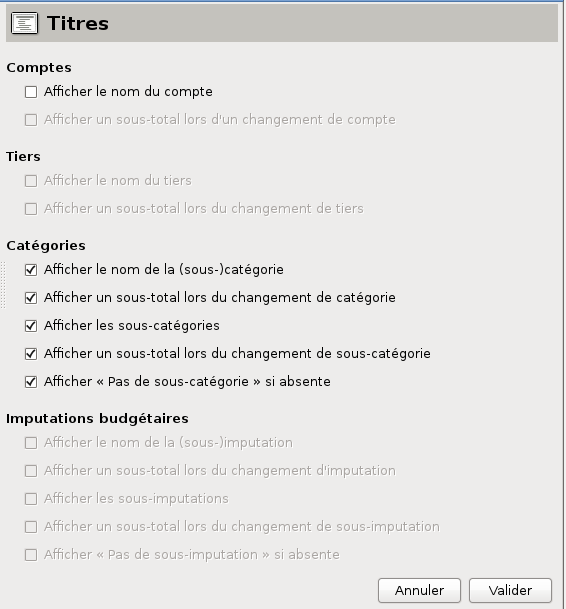
\includegraphics[scale=0.5]{image/screenshot/reportcreation_display_titles}
\end{center}
\caption{Affichage des titres}
\label{reportcreation-display-titles-img}
\end{figure}
% image centrée
\else affichés en grisé.
\fi


Pour continuer la configuration de l'affichage de vos données, passez à l'onglet suivant.


\subsection{Opérations\label{reportscreation-display-transactions}}

Dans cet onglet, vous pouvez déterminer la façon dont les opérations sélectionnées dans l'état seront affichées. Pour les afficher, cochez la case \menu{Afficher les opérations}, qui \ifIllustration  par défaut ne l'est pas\refimage{reportcreation-display-transactions-img}.

% image centrée 
\begin{figure}[htbp]
\begin{center}
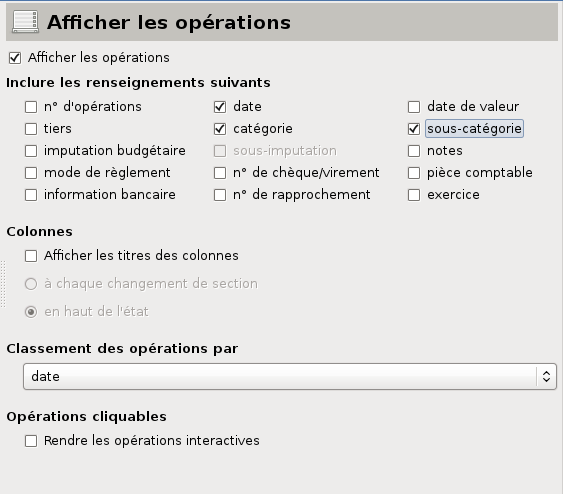
\includegraphics[scale=0.5]{image/screenshot/reportcreation_display_transactions}
\end{center}
\caption{Affichage des opérations}
\label{reportcreation-display-transactions-img}
\end{figure}
% image centrée
\else par défaut ne l'est pas.
\fi
 

\subsubsection{Inclure les renseignements suivants}

Vous pouvez choisir quelles informations seront affichées en cochant la case correspondante. Cette case a une action globale et (dés)active simultanément toutes les informations. C'est bien utile pour passer d'un état affichant les informations à un état ne les affichant pas.

Vous pouvez choisir d'afficher les renseignements suivants :

\menu{}

\begin{itemize}
	\item \menu{\no d'opération} ;
	\item \menu{tiers} ;
	\item \menu{imputation budgétaire} ;	
	\item \menu{mode de règlement} ;
	\item \menu{information bancaire} ;
	\item \menu{date} ;
	\item \menu{catégorie} ;
	\item \menu{sous-imputation budgétaire} ;
	\item \menu{\no chèque/virement} ;
	\item \menu{\no de rapprochement} ;
	\item \menu{date de valeur} ;
	\item \menu{sous-catégorie} ;
	\item \menu{notes} ;
	\item \menu{pièce comptable} ;
	\item \menu{exercice}.
\end{itemize}

Si vous vous interrogez sur l'utilité d'un \indexword{état sans opérations}\index{etat@état !sans opérations}, pensez 
que cela ne veut pas dire qu'il n'affichera rien. Vous pouvez avoir un 
état affichant uniquement les imputations et sous-imputations 
budgétaires. Cet état s'appelle \emph{Budget}.

Si vous décidez d'afficher les opérations, vous pouvez alors sélectionner
individuellement chaque information devant être affichée.

Pour plus de détails sur ces informations, voir la section \vref{transactions-list-fields}, \menu{Champs d'information et de saisie}.


\subsubsection{Colonnes\label{reportscreation-display-transactions-coltitles}}

Cliquer sur la case \menu{Afficher les titres des colonnes} vous donne l'affichage des \indexword{titres des colonnes}\index{titre !colonnes} pour chaque information affichée. Cela valide aussi les boutons :

\begin{itemize}
	\item  \menu{à chaque changement de section} (ou changement de niveau de regroupement) ;
	\item \menu{en haut de l'état}.
\end{itemize}
 
Cochez l'un de ces deux boutons selon votre besoin.

\ifIllustration
% saut de page pour titre solidaire
\newpage
\fi


\subsubsection{Classement des opérations}

Vous pouvez aussi déterminer le critère de \indexword{classement des opérations}\index{opération !classement} à l'intérieur de chaque section (ou \indexword{niveau de regroupement} \index{niveau de regroupement}). Par défaut, c'est la date de l'opération qui est sélectionnée, mais vous pouvez utiliser un autre critère de \gls{tri} dans la liste déroulante, de façon à obtenir un état trié, par exemple par tiers ou par numéro de chèque.


\subsubsection{Opérations cliquables\label{reportscreation-display-transactions-clickable}}

Enfin, vous disposez d'une case à cocher (non cochée par défaut) qui vous permet
de rendre toutes les \indexword{opérations cliquables} (ou interactives) de l'état.

Lorsque votre état terminé est validé et affiché dans le pavé des détails, si vous passez le curseur de votre souris au-dessus des opérations, leur texte passera en rouge{\couleur}, et si vous cliquez sur l'une d'entre elles, elle s'affichera dans l'onglet \menu{Opérations} du compte concerné et sera sélectionnée : la barre d'information affiche le nom du compte où est enregistrée l'opération et son solde, le panneau de navigation affiche aussi ce nom, le pavé des détails de l'état est remplacé par celui de l'onglet \menu{Opérations} de ce compte, l'opération est sélectionnée, et enfin le formulaire de saisie est ouvert et affiche le contenu de l'opération, prêt pour une modification éventuelle.

Cette fonction peut vous permettre de faire des recherches très poussées, vu la multiplicité des options de création des états. Elle peut aussi tout simplement vous permettre de corriger facilement une opération si vous constatez en lisant votre état qu'une information est erronée. Par contre, elle ralentit le temps de création de l'état, n'en abusez donc pas, à moins que votre machine soit suffisamment puissante pour vous le permettre.

% espace pour changement de thème
\vspacepdf{5mm}
Pour continuer la configuration de l'affichage de vos données, passez à l'onglet suivant.


\subsection{Devises\label{reportscreation-display-currencies}}

Les montants des opérations sont affichés dans la devise dans laquelle elles ont été enregistrées, mais les totaux sont calculés dans une seule devise, que vous pouvez choisir ici. 

Vous pouvez choisir, indépendamment, la devise pour les totaux \ifIllustration suivants\refimage{reportcreation-display-currencies-img} :
\else suivants :
\fi

\begin{itemize}
	\item totaux généraux ;
	\item tiers ;
	\item catégories ;
	\item imputations budgétaires ;
	\item comparaisons de montant.
\end{itemize} 

\ifIllustration
% image centrée
\begin{figure}[htbp]
\begin{center}
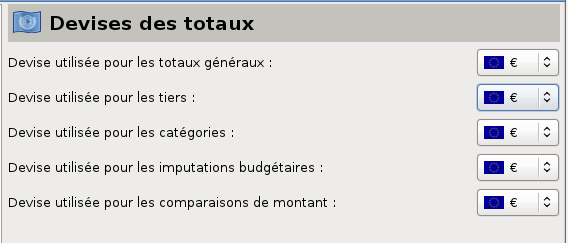
\includegraphics[scale=0.5]{image/screenshot/reportcreation_display_currencies}
\end{center}
\caption{Affichage des devises}
\label{reportcreation-display-currencies-img}
\end{figure}
% image centrée
\fi

Il faut bien sûr que vous ayez au préalable créé la devise choisie (voir la section \vref{transactions-currencies}, \menu{Gestion des devises}). 

% espace avant Attention ou Note  : 5 mm
\vspacepdf{5mm}
\textbf{Note} : Il n'est parfois pas possible de vérifier le total d'une addition car ses différentes composantes ne sont pas toutes dans la même \indexword{devise}\index{devise !différente}\dots
% espace après Attention ou Note  : 5 mm
\vspacepdf{5mm}

Il est plus que probable que vous ne choisirez la plupart du temps qu'une seule et même devise pour tous ces totaux, mais c'est une possibilité supplémentaire qu'offre là Grisbi !

% espace pour changement de thème
\vspacepdf{5mm}
Vous avez terminé la création de votre nouvel état. Pour l'enregistrer, validez-le par le bouton \menu{Valider} dans la fenêtre de création/modification. Votre nouvel état apparaît alors dans la liste des états, dans le panneau de navigation.